\chapter{Исследовательская часть}

\section{Интерфейс приложения}

На рисунке~\ref{fig:interface} представлен интерфейс приложения.

\begin{figure}[h!]
	\centering{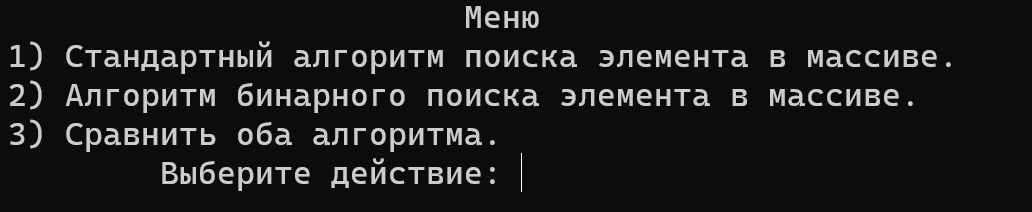
\includegraphics[scale=0.9]{photos/interface.png}}
	\caption{Интерфейс приложения}
	\label{fig:interface}
\end{figure}

\section{Технические характеристики}

Технические характеристики устройства:

\begin{itemize}
	\item операционная система --- Windows 11 Pro 64 -- разрядная система~\cite{windows};
	\item оперативная память --- 16 Гбайт;
	\item процессор --- 11th Gen Intel(R) Core(TM) i7-1165G7 с тактовой частотой 2.8 ГГц.
\end{itemize}

\section{Время выполнения реализаций алгоритмов}

На рисунке~\ref{fig:graph1} представлено сравнение времени выполнения стандартного алгоритма и алгоритма бинарного поиска элемента в массиве в лучшем случае, когда искомый элемент расположен на первом месте.
Время выполнения измерялось как среднее значение из десяти измерений.

\begin{figure}[ht!]
	\begin{center}
		\captionsetup{singlelinecheck = false, justification=centerfirst}
		\begin{tikzpicture}
			\begin{axis}[
				xlabel={Размер массива},
				ylabel={Время в секундах},
				width = 0.95\textwidth,
				height=0.5\textheight,
				xmin=0, xmax=65539,
				ymode=log, 
				legend pos=north west,
				legend style={font=\footnotesize},
				xmajorgrids=true,
				grid style=dashed,
				]
				
				\addplot[
				blue,
				semithick,
				mark = *,
				mark size = 3pt,
				thick,
				] file {graph/standart_best.csv};
				
				\addplot[
				red,
				semithick,
				mark = x,
				] file {graph/binary_best.csv};
				
				\legend{
					Стандартный алгоритм,
					Алгоритм бинарного поиска
				}
			\end{axis}
			
		\end{tikzpicture}
		\centering
		\caption{Сравнение алгоритмов по времени в лучшем случае}
		\label{fig:graph1}
	\end{center}
\end{figure}
\clearpage

На рисунке~\ref{fig:graph2} представлено сравнение времени выполнения стандартного алгоритма и алгоритма бинарного поиска элемента в массиве в худшем случае, когда искомый элемент отсутствует в массиве. 
Время выполнения было измерено как среднее значение по десяти измерениям.

\begin{figure}[ht!]
	\begin{center}
		\captionsetup{singlelinecheck = false, justification=centerfirst}
		\begin{tikzpicture}
			\begin{axis}[
				xlabel={Размер массива},
				ylabel={Время в секундах},
				width = 0.95\textwidth,
				height=0.5\textheight,
				xmin=0, xmax=65539,
				ymode=log, 
				legend pos=north west,
				legend style={font=\footnotesize},
				xmajorgrids=true,
				grid style=dashed,
				]
				
				\addplot[
				blue,
				semithick,
				mark = *,
				mark size = 3pt,
				thick,
				] file {graph/standart_worst.csv};
				
				\addplot[
				red,
				semithick,
				mark = x,
				] file {graph/binary_worst.csv};
				
				\legend{
					Стандартный алгоритм,
					Алгоритм бинарного поиска
				}
			\end{axis}
			
		\end{tikzpicture}
		\centering
		\caption{Сравнение алгоритмов по времени в худшем случае}
		\label{fig:graph2}
	\end{center}
\end{figure}
\clearpage

\section*{Вывод}

В результате исследования стандартного алгоритма поиска и алгоритма бинарного поиска с единственным сравнением для каждого медианного элемента выявлено, что в худшем случае бинарный поиск оказывается более эффективным из - за лучшей трудоемкости по сравнению со стандартным алгоритмом. 
Это связано с тем, что бинарный поиск в упорядоченном массиве делает гораздо меньше сравнений, что уменьшает общее время выполнения.

В лучшем случае бинарный поиск также демонстрирует небольшое превосходство по сравнению с стандартным алгоритмом. 
Хотя разница не столь значительна, бинарный поиск все же немного опережает стандартный алгоритм благодаря более оптимальной стратегии поиска в упорядоченном массиве.
